Figure~\ref{fig:x12345-feuer-combo} (left) shows the elliptic loci of $X_k$, $k=1,...,5$. The latter two are new results.

\begin{figure}
\centering
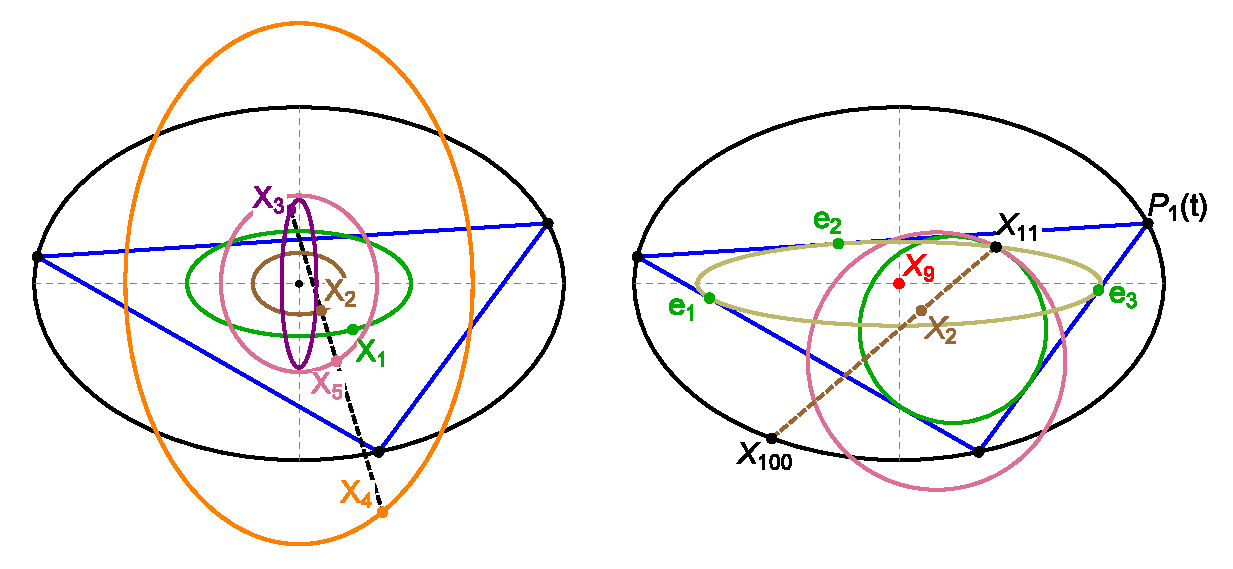
\includegraphics[width=\linewidth]{pics_1040_x12345_feuerbach_combo.eps}
\caption{\textbf{Left}: The loci of Incenter $X_1$, Barycenter $X_2$, Circumcenter $X_3$, Orthocenter $X_4$, and Center of the 9-Point Circle $X_5$ are all ellipses, \href{https://youtu.be/sMcNzcYaqtg}{Video}, \href{https://bit.ly/3opClJq}{app}. Also shown is the {\em Euler Line} (dashed black) which for any triangle, passes through all of $X_i$, $i=1...5$ \cite{mw}. \textbf{Right}: A 3-periodic orbit starting at $P_1(t)$ is shown (blue). The locus of $X_{11}$, where the Incircle (green) and 9-Point Circle (pink) meet, is the Caustic (brown), also swept by the Extouchpoints $e_i$. $X_{100}$ (double-length reflection of $X_{11}$ about $X_2$) is the EB \href{https://youtu.be/TXdg7tUl8lc}{Video}, \href{https://bit.ly/2LuARPo}{app}.}
\label{fig:x12345-feuer-combo}
\end{figure}

We have also observed that the locus of the Feuerbach Point $X_{11}$ coincides with the $N=3$ {\em Caustic}, a confocal ellipse to which the 3-periodic family is internally tangent, Appendix~\ref{app:billiards}. Additionally, the locus of $X_{100}$, the Anticomplement\footnote{Double-length reflection about the Centroid $X_2$.} of $X_{11}$ is the EB boundary. These phenomena appear in Figure~\ref{fig:x12345-feuer-combo} (right).

Indeed, some these facts will be known to triangle specialists if one regards the EB as the circumellipse centered on the Mittenpunkt $X_9$ \cite[X(9)]{etc} and \cite{dekov14}. For example, a full 57 Triangle Centers lie on said circumellipse. An animation of some of these points is viewable in \cite[pl\#10]{dsr_playlist_2020}.

\begin{figure}
 \begin{minipage}{\textwidth}
    \centering
    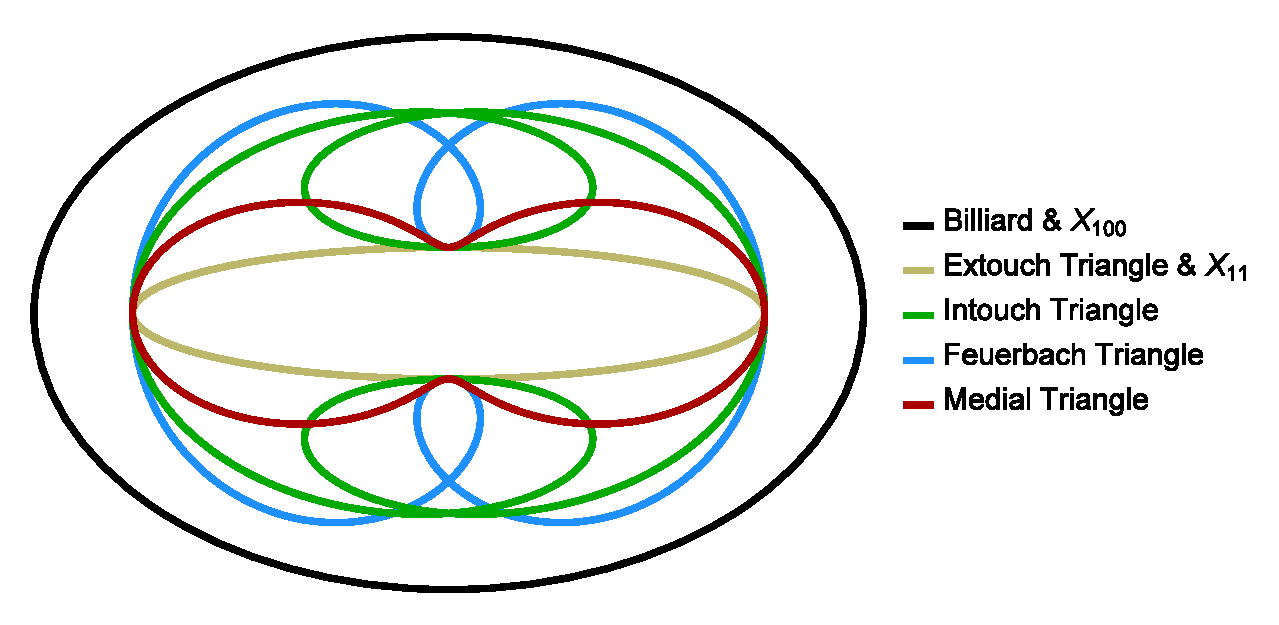
\includegraphics[width=.85\textwidth]{pics_1050_non_elliptic.eps}
    \caption[blablabla]{Loci generated by the vertices of selected orbit-Derived Triangles, namely: the Intouch (green), Feuerbach\footnote{Not to be confused with the Feuerbach Point $X_{11}$. The Feuerbach Triangle has vertices at the three contact points of the 9-point Circle with the Excircles \cite{mw}.} (blue), and Medial (red) Triangles are non-elliptic. However, those of the Extouch Triangle (brown), are identical to the $N=3$ Caustic (a curve also swept by $X_{11}$). Not shown is the locus of the Excentral Triangle, an ellipse similar to a rotated copy of the Incenter locus. \href{https://bit.ly/2MMH9e5}{app},
    \href{https://youtu.be/9xU6T7hQMzs}{Video 1}, \href{https://youtu.be/Xxr1DUo19_w}{Video 2}, \href{https://youtu.be/TXdg7tUl8lc}{Video 3}, \href{https://youtu.be/OGvCQbYqJyI}{Video 4}.}
    % tem q ficar aqui dentro do minipage!
    \label{fig:non-elliptic-vertex}
    \end{minipage}
\end{figure}

Additionally, a few  observations have been made \cite{reznik2020-intelligencer} about the loci of vertices of orbit-derived triangles (see Appendix~\ref{app:derived-tris}), some of which are elliptic and others non, illustrated in Figure~\ref{fig:non-elliptic-vertex}.